%%%%%%%%%%%%%%%%%%%%%%%%%%%%%%%%%%%%%%%%%%%%%%%%%%%%%%%%%%%%%%%%%%%%%%%%%%%%%%%%
% AMS Beamer series / Bologna FC / Template
% Andrea Omicini
% Alma Mater Studiorum - Università di Bologna
% mailto:andrea.omicini@unibo.it
%%%%%%%%%%%%%%%%%%%%%%%%%%%%%%%%%%%%%%%%%%%%%%%%%%%%%%%%%%%%%%%%%%%%%%%%%%%%%%%%
%\documentclass[handout]{beamer}\mode<handout>{\usetheme{default}}
%
\documentclass[presentation, 9pt]{beamer}\mode<presentation>{\usetheme{AMSBolognaFC}}
%\documentclass[handout]{beamer}\mode<handout>{\usetheme{AMSBolognaFC}}
%%%%%%%%%%%%%%%%%%%%%%%%%%%%%%%%%%%%%%%%%%%%%%%%%%%%%%%%%%%%%%%%%%%%%%%%%%%%%%%%
\usepackage[T1]{fontenc}
\usepackage{wasysym}
\usepackage{amsmath,blkarray}
\usepackage{soul}
\usepackage[minted,most]{tcolorbox}
\usepackage{centernot}
\usepackage{fontawesome}
\usepackage{fancyvrb}
\usepackage{hyperref}
\usepackage{multicol}
\setminted[scala]{fontsize=\small,frame=lines,baselinestretch=1,obeytabs=true, tabsize=2}
\setminted[yaml]{fontsize=\large,frame=lines,linenos,baselinestretch=1,obeytabs=true, tabsize=2}
\usepackage[ddmmyyyy]{datetime}
\setminted{fontsize=\footnotesize}
\renewcommand{\dateseparator}{}
%\renewcommand{\thefootnote}{\fnsymbol{footnote}}
\newcommand{\version}{1}

\usepackage[
	%backend=biber,
	backend=bibtex,
%	citestyle=authoryear-icomp,
%	maxcitenames=1,
	bibstyle=numeric,
	style=ieee]{biblatex}

	\makeatletter

%\addbibresource{biblio.bib}

\bibliography{biblio}


\newcommand\extrafootertext[1]{%
    \bgroup
    \renewcommand\thefootnote{\fnsymbol{footnote}}%
    \renewcommand\thempfootnote{\fnsymbol{mpfootnote}}%
    \footnotetext[0]{#1}%
    \egroup
}

\newcommand{\citeinslide}[1]{\cite{#1}\extrafootertext{\scriptsize\cite{#1} \fullcite{#1}}}


%%%%%%%%%%%%%%%%%%%%%%%%%%%%%%%%%%%%%%%%%%%%%%%%%%%%%%%%%%%%%%%%%%%%%%%%%%%%%%%%
\title[AP -- Implementations overview]
{Aggregate Programming -- Implementations overview}
%
%
\author[\sspeaker{Aguzzi}]
{\speaker{Gianluca Aguzzi} \href{mailto:gianluca.aguzzi@unibo.it}{gianluca.aguzzi@unibo.it} }
\institute[DISI, Univ.\ Bologna]
{%Dipartimento di Informatica -- Scienza e Ingegneria (DISI)\\
\textsc{Alma Mater Studiorum} -- Universit{\`a} di Bologna \\[0.1cm]
%\textbf{Talk @} \bold{International Conference on Autonomic Computing and Self-Organizing Systems (ACSOS)}\\[0.15cm]
%
\includegraphics[width=0.15\textwidth]{img/qr-code-today.png}
}
%
\renewcommand{\dateseparator}{/}
\date[\today]{\today}
%

%%%%%%%%%%%%%%%%%%%%%%%%%%%%%%%%%%%%%%%%%%%%%%%%%%%%%%%%%%%%%%%%%%%%%%%%%%%%%%%%



\lstdefinelanguage{scala}{
  keywords={abstract,case,catch,class,def,%
    do,else,extends,false,final,finally,%
    for,if,implicit,import,match,mixin,%
    new,null,object,override,package,%
    private,protected,requires,return,sealed,%
    super,this,throw,trait,true,try,lazy,%
    type,val,var,while,with,yield,forSome},
  otherkeywords={=>,<-,<\%,<:,>:,\#},
  sensitive=true,
  morecomment=[l]{//},
  morecomment=[n]{/*}{*/},
  morestring=[b]",
  morestring=[b]',
  morestring=[b]""",
  basicstyle=\lst@ifdisplaystyle\footnotesize\fi\ttfamily,
  emphstyle=\bfseries
}
\definecolor{ddarkgreen}{rgb}{0,0.5,0}
\lstdefinelanguage{scafi}{frame=single,basewidth=0.5em,language={scala},
keywordstyle=\color{blue}\textbf, commentstyle=\color{ddarkgreen},
keywordstyle=[2]\color{red}\textbf, keywords=[2]{rep,nbr,foldhood,foldhoodPlus,aggregate,branch,spawn},
keywordstyle=[3]\color{gray}, keywords=[3]{Me,AroundMe,Everywhere,Forever}, %,@@,@@@
keywordstyle=[4]\color{red}\textbf, keywords=[4]{in,out,rd},
keywordstyle=[5]\color{violet}, keywords=[5]{evolve,when,andNext,workflow,C,gossip},
keywordstyle=[6]\color{orange}, keywords=[6]{Available,Serving,Done,Waiting,Removing}}

\newcommand{\hsplit}[2]{
\begin{minipage}{0.48\textwidth}
#1
\end{minipage}
\hfill
\begin{minipage}{0.48\textwidth}
#2
\end{minipage}
}
\newcommand{\hsplits}[4]{
\begin{minipage}{#1\textwidth}
#3
\end{minipage}
\hfill
\begin{minipage}{#2\textwidth}
#4
\end{minipage}
}

\newcommand{\lbl}[1]{\textbf{\textcolor{gray!90!white}{#1}}}
\newcommand{\enf}[1]{{\textcolor{red}{#1}}}
\newcommand{\bo}[1]{\textbf{#1}}

\newcommand{\imgh}[2]{
\begin{figure}
\centering
\includegraphics[width=#1\textwidth]{img/#2}
\end{figure}
}
\newcommand{\imgv}[2]{
\begin{figure}
\centering
\includegraphics[height=#1\textheight]{img/#2}
\end{figure}
}

\newtcblisting{mycode}[3]{%
  boxsep=0pt,
  boxrule=0pt,
  arc=1mm, 
  left=1mm,
  %auto outer arc,
  size=fbox,%tight,
  %colframe=blue!40!black, colframe=black!30!white,
  %colbacktitle=blue!80!white,
  colback=blue!5,
  %toprule=0.1mm, bottomrule=0.1mm, rightrule=0.1mm, leftrule=1mm, 
  listing only,
  listing options={language=scafi, alsoletter={-},
    backgroundcolor={},
  	columns=fullflexible,
  	lineskip={-1.5pt},
  	xleftmargin=0px,
  	belowskip={0px},
  	aboveskip={0px},
  	frame=none,
  	#2
  },
  title={#3},#1
}
\lstdefinestyle{s}{basicstyle=\ttfamily\footnotesize}
\lstdefinestyle{ss}{basicstyle=\ttfamily\scriptsize}
\lstdefinestyle{sss}{basicstyle=\ttfamily\tiny}
\lstdefinestyle{conf}{language={},morecomment=[l][\color{darkgreen}]{\#},
basicstyle=\ttfamily\scriptsize}

\newcommand{\question}[1]{\textcolor{darkgray}{\emph{\bo{#1}}}}
\newcommand{\refslide}[1]{Slide~\ref{#1}}

\begin{document}
%%%%%%%%%%%%%%%%%%%%%%%%%%%%%%%%%%%%%%%%%%%%%%%%%%%%%%%%%%%%%%%%%%%%%%%%%%%%%%%%
%!TeX root = presentation-2024-ap-toolchain.tex
%%% Syntax

\newcommand{\FieldS}[0]{\mathcal{F}}
\newcommand{\EventS}[0]{\mathcal{E}}
\newcommand{\eventS}[0]{E}
\newcommand{\timeS}[0]{t}
\newcommand{\posS}[0]{p}
\newcommand{\event}[3]{\langle #1,#2,#3\rangle}
\newcommand{\devF}[1]{\deviceId_{#1}}
\newcommand{\timeF}[1]{\timeS_{#1}}
\newcommand{\posF}[1]{\posS_{#1}}
\newcommand{\domS}[0]{D}
\newcommand{\DomS}[0]{\mathcal{D}}
\newcommand{\DomDevF}[2]{#1(#2)}
\newcommand{\DomTimeF}[2]{#1(#2)}
\newcommand{\DomMTimeF}[2]{#1^{-}(#2)}
\newcommand{\DomDomF}[2]{#1(#2)}
\newcommand{\DomDevTimeF}[3]{#1(#2,#3)}
\newcommand{\DomDevMTimeF}[3]{#1^{-}(#2,#3)}

\newcommand{\feS}[0]{\Phi}
\newcommand{\setVS}[0]{\textbf{V}}
\newcommand{\setTS}[0]{\textbf{T}}
\newcommand{\setCS}[0]{\textbf{C}}

\newcommand\pto{\mathrel{\ooalign{\hfil$\mapstochar$\hfil\cr$\to$\cr}}}

\newcommand{\neighbour}[2]{\textit{neigh}(#1,#2)}

\newcommand{\denot}[1]{\mathcal{E}\llbracket{#1}\rrbracket}
\newcommand{\denotapp}[2]{\denot{#1}_{#2}}
\newcommand{\denotappsub}[3]{\denot{#1}_{#2}^{#3}}
\newcommand{\denotfun}[3]{\mathcal{L}\llbracket{#1}\rrbracket_{#2}^{#3}}
\newcommand{\denottype}[1]{\mathcal{T}\llbracket{#1}\rrbracket}
\newcommand{\denotexp}[3]{\mathcal{E}\llbracket{#1}\rrbracket_{#2}^{#3}}
\newcommand{\denotf}[2]{\lambda #1.#2}

\newcommand{\dvalue}[0]{V}

\newcommand{\myeval}[4]{\epsilon(#1,#2,#3,#4)}

\newcommand{\fiecomp}[2]{#1[#2]}


\newcommand{\BNFcce}{{\bf ::=}}
\newcommand{\BNFmid}{\;\bigr\rvert\;}

\newcommand{\PROGRAM}{\texttt{P}}
\newcommand{\FUNCTION}{\texttt{F}}
\newcommand{\e}{\texttt{e}}
\newcommand{\fname}{\texttt{f}}
\newcommand{\xname}{\texttt{x}}
\newcommand{\yname}{\texttt{y}}
\newcommand{\oname}{\texttt{o}}
\newcommand{\pe}{\texttt{p}} % pure expression
\newcommand{\we}{\texttt{w}} % variable or (local) value




\newcommand{\asuper}{\texttt{s}}
\newcommand{\avalue}{\texttt{v}}
\newcommand{\bvalue}{\textit{b}}
\newcommand{\obvalue}{\option{\bvalue}}
\newcommand{\lvalue}{\texttt{l}}
\newcommand{\olvalue}{\option{\lvalue}}
\newcommand{\nvalue}{\texttt{n}}
\newcommand{\tvalue}{\texttt{t}}
\newcommand{\hvalue}{\texttt{h}}
\newcommand{\fvalue}{\phi}
\newcommand{\nolabel}{\_}
\newcommand{\fdom}[1]{\textit{dom}(#1)}
\newcommand{\oexec}{\epsilon}

\newcommand{\brvalue}{\textit{b}}
\newcommand{\obrvalue}{\option{\brvalue}}
\newcommand{\lrvalue}{\textit{l}}
\newcommand{\olrvalue}{\option{\lrvalue}}

\newcommand{\tvalueExt}[1]{(\lvalue_1,\ldots,\lvalue_{#1})}
\newcommand{\fvalueExt}[2]{\{#1\mapsto #2\}}
\newcommand{\fvalueOne}[2]{\{#1\mapsto #2\}}
\newcommand{\fvalueWrap}[1]{\{#1\}}
\newcommand{\fvaluewrapped}[2]{#1\mapsto #2}
\newcommand{\fvalues}[2]{#1\mapsto #2}
%\newcommand{\memslot}[2]{\{#1:=#2\}}
\newcommand{\memslot}[2]{#1:=#2}
\newcommand{\treeslot}[2]{#1\mapsto #2}
\newcommand{\emptyL}{\bullet}

\newcommand{\avalueSet}{\mathcal{V}}
\newcommand{\lvalueSet}{\mathcal{L}}
\newcommand{\nvalueSet}{\mathcal{N}}
\newcommand{\tvalueSet}{\mathcal{T}}
\newcommand{\hvalueSet}{\mathcal{H}}
\newcommand{\fvalueSet}{\Phi}
% Keywords
\newcommand{\defK}{\texttt{def}}
\newcommand{\nbrK}{\texttt{nbr}}
\newcommand{\repK}{\texttt{rep}}
\newcommand{\ifK}{\texttt{if}}

\newcommand{\tname}{\texttt{t}}

\newcommand{\ltrue}{\textit{t}}
\newcommand{\lfalse}{\textit{f}}


%%% Runtime Syntax

\newcommand{\wildcard}{{\cdots}} %%% non intresting syntact element
%\newcommand{\option}[1]{{{#1}_\mathit{opt}}} %%% optional syntact element
\newcommand{\option}[1]{\mathring{#1}} %%% optional
\newcommand{\evaluatedPlace}{{\place_\mathit{top}}} %%% optional syntact element
%%%\newcommand{\re}{\textit{r}} %%% runtime expression
\newcommand{\re}{\textit{a}} %%% runtime expression
\newcommand{\rv}{\textit{v}} %%% runtime value
\newcommand{\lre}{\textit{e}} %%% labeled runtime expression
\newcommand{\olre}{\option{\lre}} %%% optional labeled runtime expression
%%%\newcommand{\orv}{\textit{w}}  %%% optional runtime value
\newcommand{\orv}{\option{\rv}}  %%% optional runtime value
\newcommand{\ob}{\textit{b}}  %%% optional body
\newcommand{\Env}{\Gamma}
\newcommand{\emptyEnv}{\bullet}
\newcommand{\Trees}{\Theta}
\newcommand{\emptyTrees}{\bullet}
\newcommand{\labelled}[2]{#1\!\!\cdot\!\!{#2}}
\newcommand{\labelledsmall}[2]{#1\cdot{#2}}
\newcommand{\labelledC}[2]{#1^{#2}}
\newcommand{\labelledCsmall}[2]{#1^{#2}}

\newcommand{\he}{h} %%%  local value or runtime expression
\newcommand{\ohe}{\option{\he}} %%% optional local value or runtime expression
\newcommand{\ue}{\textit{u}} %%% unevaluated runtime expression
\newcommand{\uhe}{\option{\ue}} %%% optional unevaluated runtime expression

\newcommand{\unfoldK}{\texttt{unfold}}

\newcommand{\newopsem}[5]{#1;#2;#3\vdash #4\rightarrow #5}
\newcommand{\opsem}[4]{#1;#2\vdash #3\rightarrow #4}
\newcommand{\opsemmany}[4]{#1;#2\vdash #3\rightarrow^* #4}
\newcommand{\opsemNF}[3]{#1;#2\vdash #3\not\rightarrow}

\newcommand{\self}{\texttt{self}}

%%% Alignment contexts

\newcommand{\actx}{\mathbb{A}}
\newcommand{\matches}{::}

%%% Contexts

\newcommand{\ctxapp}[2]{#1[#2]}
\newcommand{\ctxappfull}[3]{\ctxapp{#1}{#2}\langle #3\rangle}
\newcommand{\ctx}{\mathbb{C}}
\newcommand{\ctxr}{\mathbb{R}}
\newcommand{\ctxf}{\mathbb{N}}
\newcommand{\ctxc}{\mathbb{C}}
\newcommand{\ctxrt}{\mathbb{RT}}
\newcommand{\ctxt}{\mathbb{T}}
\newcommand{\ctxre}{\mathbb{RE}}
\newcommand{\ctxe}{\mathbb{E}}
\newcommand{\hole}{[]}
\newcommand{\place}{\langle\rangle}
\newcommand{\placefilled}[1]{\langle #1\rangle}
\newcommand{\inversectx}[2]{\spi{#1}(#2)}
\newcommand{\spi}[1]{\pi_{#1}}
\newcommand{\erase}[1]{|#1|}

\newcommand{\transition}[3]{
  \begin{array}{l@{\;}c}
    \stackrel{~}{{\tiny \textrm{[#1]}}} & #2 \\ \hline
    \multicolumn{2}{c}{#3}
  \end{array}
}
\newcommand{\transitiontwoprec}[4]{
  \begin{array}{l@{\qquad}c}
    & #2\\
    {\tiny \textrm{[#1]}} & #3 \\ \hline
    \multicolumn{2}{c}{#4}
  \end{array}
}
\newcommand{\nulltransition}[2]{
  \transition{#1}{}{#2}
}

\newcommand{\smallerskiptransition}{\\[-4pt]}
\newcommand{\smallskiptransition}{\\[0pt]}
\newcommand{\skipreduction}{\\}
\newcommand{\skiptransition}{\\[10pt]}
\newcommand{\bigskiptransition}{\\[15pt]}

\newcommand{\sta}{\textit{s}}
\newcommand{\stat}[4]{\langle#1,#2,#3,#4\rangle}
\newcommand{\topStat}[3]{\langle#1,#2,#3\rangle}
\newcommand{\tstat}[5]{#1\!::\!\langle #2,#3,#4,#5\rangle}
\newcommand{\msg}[2]{\{#1\rhd #2\}}
\newcommand{\fullmsg}[3]{#1:#2\rhd #3}
\newcommand{\sys}{\textit{N}}
\newcommand{\opar}{\;||\;}
\newcommand{\opard}{\oplus}
\newcommand{\lab}{\lambda}
\newcommand{\labtau}[1]{#1:\tau}
\newcommand{\labstart}[2]{#1\uparrow #2}
\newcommand{\labstop}[3]{#1\downarrow(#3) #2}
\newcommand{\upd}[2]{#1[#2]}
\newcommand{\replace}[2]{#2\rhd #1}
\newcommand{\proj}[2]{{#1}|_{#2}}
\newcommand{\topo}{\varSigma}
\newcommand{\envmap}[2]{\{#1\mapsto #2\}}

\newcommand{\fromMsg}[2]{\mathit{from}(#1,#2)}
\newcommand{\toMsg}[2]{\mathit{to}(#1,#2)}

\newcommand{\initNAME}{\textit{init}}
\newcommand{\init}[1]{\initNAME(#1)}
\newcommand{\ruleNameSize}[1]{{\scriptsize #1}}

\newcommand{\shadow}[1]{{\it \textcolor{gray}{#1}}} % inline comment

% Code highlighting
\newcommand{\il}[1]{{\it \textcolor{gray}{;; #1}}} % inline comment
\newcommand{\km}[1]{{\bf \textcolor{red}{#1}}} % key mechanism primitives
\newcommand{\fn}[1]{\textcolor{blue}{#1}} % function calls
\newcommand{\pr}[1]{\textcolor{magenta}{#1}} % primitives
\newcommand{\bk}[1]{{\bf\fn{#1}}} % primitives

%values

\newcommand{\somevalue}{\texttt{w}}
\newcommand{\anyvalue}{\texttt{v}}
\newcommand{\anyvaluealt}{\texttt{u}}
\newcommand{\anyvaluebis}{\texttt{w}}
\newcommand{\anyvalueInNC}[2]{\anyvalue_{#1 (\textrm{in }#2)}}
\newcommand{\nullvalue}{\texttt{null}}
\newcommand{\propervalue}{\texttt{w}}
\newcommand{\numvalue}{\texttt{n}}
\newcommand{\stringvalue}{\texttt{s}}
\newcommand{\boolvalue}{\texttt{b}}
\newcommand{\groundvalue}{\texttt{g}}
\newcommand{\pairvalue}[2]{\langle#1,#2\rangle}


%sensors
%\newcommand{\snsname}{\texttt{\#sns}}
%\newcommand{\snsname}{s}
\newcommand{\snsname}{\texttt{Sns}}

%operators and functions
\newcommand{\pname}{\texttt{p}}
\newcommand{\main}{\texttt{main}}

%constructs
\newcommand{\spreadK}{\texttt{spread}}
\newcommand{\spreadTwo}[2]{\spreadK(#1:#2(*))}
%\newcommand{\spreadThree}[3]{\spreadK(#1\wedge#2(*,#3))}
\newcommand{\starK}{\texttt{@}}
\newcommand{\progK}[2]{#1(\starK,#2)}
\newcommand{\spreadThree}[3]{\{#1:\progK{#2}{#3}\}}

\newcommand{\saaK}{\texttt{grd}}
\newcommand{\saaTwo}[2]{\saaK(#1,#2)}
\newcommand{\saaThree}[3]{\saaK(#1,#2,#3)}

%typing functions and predicates
\newcommand{\lengthOf}[1]{\textit{length}(#1)}
\newcommand{\sizeOf}[1]{\textit{size}(#1)}
\newcommand{\signature}{\textit{signature}}
\newcommand{\signatureOf}[1]{\signature(#1)}
\newcommand{\bsWFTE}[4]{\textit{WFTE}(#1,#2,#3,#4)}

%types
\newcommand{\anytype}{\texttt{T}}
\newcommand{\nulltype}{\texttt{any}}
\newcommand{\numtype}{\texttt{mumber}}
\newcommand{\booltype}{\texttt{boolean}}
\newcommand{\stringtype}{\texttt{string}}
\newcommand{\pairtype}[2]{(#1\star#2)}

%type semantics
\newcommand{\lsempar}{[\![}
\newcommand{\rsempar}{]\!]}
\newcommand{\semOf}[1]{\lsempar{#1}\rsempar}
\newcommand{\lowerBound}{\textstyle{\bigwedge}}
\newcommand{\lowerBoundWith}[1]{\lowerBound_{#1}}

\newcommand{\suitableProse}{locally noetherian}
\newcommand{\suitableTypeText}{lnoe}
%\newcommand{\SuitableTypeText}{Noe}
\newcommand{\suitableType}{\suitableTypeText}
\newcommand{\suitableTypeOf}[1]{\suitableType(#1)}
\newcommand{\suitableOpText}{suitable}
\newcommand{\SuitableOpText}{stabilising}
\newcommand{\suitableOp}{\SuitableOpText}
\newcommand{\suitableOpOf}[1]{\suitableOp(#1)}


\newcommand{\wfLt}{<}
\newcommand{\wfLtOf}[1]{\wfLt_{#1}}
\newcommand{\wfLe}{\le}
\newcommand{\wfLeOf}[1]{\wfLe_{#1}}

\newcommand{\wfGt}{>}
\newcommand{\wfGtOf}[1]{\wfGt_{#1}}
\newcommand{\wfGe}{\ge}
\newcommand{\wfGeOf}[1]{\wfGe_{#1}}

\newcommand{\neginf}{\texttt{bottom}}
\newcommand{\neginfOf}[1]{\neginf(#1)}
\newcommand{\posinf}{\texttt{top}}
\newcommand{\posinfOf}[1]{\posinf(#1)}
\newcommand{\initial}{\texttt{default}}
\newcommand{\initialOf}[1]{\initial(#1)}
\newcommand{\topvalue}{\top}
\newcommand{\topvalueOf}[1]{\topvalue_{#1}}
\newcommand{\TypeDouble}{\texttt{Double}}
\newcommand{\topvalueOfDouble}[1]{\topvalue_{#1}}

%semantic functions and predicates
\newcommand{\minimize}{\textit{min}}
\newcommand{\minimizeOf}[1]{\minimize_{#1}}
\newcommand{\dom}{\textit{dom}}
\newcommand{\domOf}[1]{\dom(#1)}
\newcommand{\noetherian}{\textit{noetherian}}
\newcommand{\noetherianOf}[1]{\noetherianOf(#1)}
\newcommand{\noetherianOrd}{<}
\newcommand{\noetherianOrdOf}[1]{\noetherianOrd_{#1}}
\newcommand{\progressive}{\textit{Progressive}}
\newcommand{\progressiveOf}[1]{\progressive(#1)}
\newcommand{\sense}[2]{#1(#2)}

%small-step network operational semantic
\newcommand{\netframe}{\Envi}
\newcommand{\mknetframe}[3]{(#1,#2,#3)}
\newcommand{\netframeName}{\textit{environment}}
\newcommand{\netframeOf}[1]{\netframeName(#1)}
\newcommand{\stablencOf}[1]{R_{#1}}
%\newcommand{\stablencOf}[1]{\textit{snc}(#1)}

\newcommand{\deviceIdSet}{\textbf{D}}
\newcommand{\nodeSubSet}{\textbf{C}}
\newcommand{\stableNodeSet}{\textbf{S}}
\newcommand{\network}{\Cfg}
\newcommand{\netRestrict}[2]{#1|_{#2}}
\newcommand{\initialNetwork}{\mathcal{I}}
\newcommand{\stableNetwork}{R}
\newcommand{\mkgraph}[2]{(#1,#2)}
\newcommand{\mknetwork}[4]{(#1,#2,#4,#3)}
\newcommand{\nodeSet}{\textbf{N}}
\newcommand{\edgeSet}{\textbf{E}}
\newcommand{\stateMap}{\Delta}
\newcommand{\statePair}[2]{(#1,#2)}
\newcommand{\stateMapPair}[2]{(#1,#2)}
\newcommand{\snsFunMap}{\Sigma}
\newcommand{\topSnsFun}{\tau}
\newcommand{\InitialSnsFun}[1]{\textit{Initial}(#1)}
%\newcommand{\topSnsFun}{\snsFun_{\posinf}}
\newcommand{\snsFun}{\sigma}
\newcommand{\snsFunFor}[1]{\snsFun_{#1}}
\newcommand{\snsFunOf}[1]{\snsFunMap(#1)}
\newcommand{\snsFunMapPair}[2]{(#1,#2)}
\newcommand{\snsFunPair}[2]{(#1,#2)}
\newcommand{\mkedge}[2]{(#1,#2)}
\newcommand{\neigh}{\textit{neighbours}}
\newcommand{\neighOfIn}[2]{\neigh(#1,#2)}
\newcommand{\neighTE}{\textit{nvte}}
\newcommand{\neighTEOfIn}[3]{\neighTE(#1,#2,#3)}
\newcommand{\Disconnected}{\textit{Disconnected}}
\newcommand{\DisconnectedOfIn}[2]{\Disconnected(#1,#2)}
\newcommand{\codom}{\textit{codom}}
\newcommand{\codomOf}[1]{\codom(#1)}
\newcommand{\frontier}{\textit{frontier}}
\newcommand{\frontierOfIn}[2]{\frontier_{#1}(#2)}
\newcommand{\netopsemarrow}{\longrightarrow}
\newcommand{\netopsemarrowWith}[1]{\longrightarrow_{#1}}
\newcommand{\netopsemarrowStar}{\netopsemarrow^{\star}}
\newcommand{\netopsemarrowPlus}{\netopsemarrow^{+}}
\newcommand{\netopsem}[2]{#1\netopsemarrow#2}
\newcommand{\netopsemStar}[2]{#1\netopsemarrowStar#2}
\newcommand{\netopsemPlus}[2]{#1\netopsemarrowPlus#2}
\newcommand{\netopsemWith}[3]{#2\netopsemarrowWith{#1}#3}
\newcommand{\netopsemWithStar}[3]{#2\netopsemarrowWith{#1}#3}
\newcommand{\netopsemWithPlus}[3]{#2\netopsemarrowWith{#1}#3}
\newcommand{\netopsemRule}[3]{\surfaceTyping{#1}{#2}{#3}}
\newcommand{\nullnetopsemRule}[2]{\nullsurfaceTyping{#1}{#2}}
%\newcommand{\evaluationTrace}{\theta}
\newcommand{\initialvtree}{\theta_{\main}}
\newcommand{\vtree}{\theta}
\newcommand{\vtreealt}{\eta}
\newcommand{\vtreeInNC}[2]{\theta_{#1( \textrm{in }#2)}}
\newcommand{\initialTraceFor}[1]{\evaluationTrace_{#1}}
\newcommand{\traceFor}[4]{\evaluationTrace_{(#1,#2,#3,#4)}}
\newcommand{\donotcare}{\_}
\newcommand{\ruleName}{\textbf{r}}
\newcommand{\ruleNameSet}{\textbf{R}}
\newcommand{\senstate}{\sigma}
\newcommand{\genmap}[2]{#1\rhd#2}


\newcommand{\act}{\textit{act}}
\newcommand{\envact}{\textit{env}}
\newcommand{\netArr}{\rightarrow}
\newcommand{\netRed}[2]{#1\netArr#2}
\newcommand{\netArrAct}{\stackrel{\act}{\netArr}}
\newcommand{\netRedAct}[2]{#1\netArrAct#2}
\newcommand{\netArrWithAct}[1]{\stackrel{#1}{\netArr}}
\newcommand{\trueUpd}{\textsf{true}}
\newcommand{\falseUpd}{\textsf{false}}
\newcommand{\isUpd}{\textsf{b}}

\newcommand{\netArrStar}{\Longrightarrow}
%\newcommand{\netArrStar}{\longrightarrow^{\star}}
\newcommand{\netArrActStar}{\stackrel{\overline{\act}}{\netArrStar}}
%\newcommand{\netArrActStar}{\xrightarrow{\overline{\act}}^{\star}}
\newcommand{\netArrWithActStar}[1]{\stackrel{#1}{\netArrStar}}
%\newcommand{\netArrWithActStar}[1]{\xrightarrow{#1}^{\star}}

\newcommand{\netRedStar}[2]{#1\netArrStar#2}
\newcommand{\netRedWithActStar}[3]{#2\netArrWithActStar{#1}#3}

\newcommand{\pres}{\not\epsilon}
\newcommand{\netArrPres}{\netArr_{\pres}}
\newcommand{\netArrPresStar}{\netArrStar}
\newcommand{\netArrActPres}{\netArrAct}
\newcommand{\netArrActPresStar}{\netArrActStar}
\newcommand{\netArrWithActPresStar}[1]{\stackrel{#1}{\netArrStar}}

\newcommand{\firing}{\textit{firing}}
\newcommand{\fair}{\textit{fair}}
\newcommand{\Fair}{\textit{Fair}}

\newcommand{\fairsym}{\star}
\newcommand{\netArrFairStar}{\netArrStar_{\fairsym}}
\newcommand{\netArrActFairStar}{\netArrActStar_{\fairsym}}
\newcommand{\netArrFairStarN}[1]{\netArrStar_{#1}}
\newcommand{\netArrActFairStarN}[1]{\netArrActStar_{#1}}
\newcommand{\netRedFairStar}[2]{#1\netArrFairStar#2}
\newcommand{\netRedActFairStar}[2]{#1\netArrActFairStar#2}
\newcommand{\netRedActFairStarN}[3]{#2\netArrActFairStarN{#1}#3}


\newcommand{\actDevIn}{\textsf{di}}
%\newcommand{\actDevInOf}[1]{\actDevIn(#1)}
\newcommand{\actDevInOf}[1]{\envact}
\newcommand{\netArrDevInOf}[1]{\netArrWithAct{\actDevInOf{#1}}}
\newcommand{\netRedDevInOf}[3]{#2\netArrWithAct{\actDevInOf{#1}}#3}

\newcommand{\actDevOut}{\textsf{do}}
%\newcommand{\actDevOutOf}[1]{\actDevOut(#1)}
\newcommand{\actDevOutOf}[1]{\envact}
\newcommand{\netArrDevOutOf}[1]{\netArrWithAct{\actDevOutOf{#1}}}
\newcommand{\netRedDevOutOf}[3]{#2\netArrWithAct{\actDevOutOf{#1}}#3}

\newcommand{\actEdgeIn}{\textsf{ei}}
%\newcommand{\actEdgeInOf}[1]{\actEdgeIn(#1)}
\newcommand{\actEdgeInOf}[1]{\envact}
\newcommand{\netArrEdgeInOf}[1]{\netArrWithAct{\actEdgeInOf{#1}}}
\newcommand{\netRedEdgeInOf}[3]{#2\netArrWithAct{\actEdgeInOf{#1}}#3}

\newcommand{\actEdgeOut}{\textsf{eo}}
%\newcommand{\actEdgeOutOf}[1]{\actEdgeOut(#1)}
\newcommand{\actEdgeOutOf}[1]{\envact}
\newcommand{\netArrEdgeOutOf}[1]{\netArrWithAct{\actEdgeOutOf{#1}}}
\newcommand{\netRedEdgeOutOf}[3]{#2\netArrWithAct{\actEdgeOutOf{#1}}#3}

\newcommand{\actSnsUpd}{\textsf{su}}
%\newcommand{\actSnsUpdOf}[1]{\actSnsUpd(#1)}
\newcommand{\actSnsUpdOf}[1]{\envact}
\newcommand{\netArrSnsUpdOf}[1]{\netArrWithAct{\actSnsUpdOf{#1}}}
\newcommand{\netRedSnsUpdOf}[3]{#2\netArrWithAct{\actSnsUpdOf{#1}}#3}

\newcommand{\actDevUpd}{\textsf{df}}
%\newcommand{\actDevUpdOf}[1]{\actDevUpd(#1)}
\newcommand{\actDevUpdOf}[1]{#1}
\newcommand{\netArrDevUpdOf}[1]{\netArrWithAct{\actDevUpdOf{#1}}}
\newcommand{\netRedDevUpdOf}[3]{#2\netArrWithAct{\actDevUpdOf{#1}}#3}

%big-step device operational semantic
\newcommand{\resPair}[2]{#1,\,#2}
\newcommand{\emain}{\e_{\main}}
\newcommand{\opFun}{\epsilon}
%\newcommand{\opFunOf}[1]{\opFun_{#1}}
\newcommand{\opFunOf}[1]{\semOf{#1}}
\newcommand{\opApply}[2]{#1(#2)}
\newcommand{\neighSet}{\Theta}
\newcommand{\labe}{\texttt{l}}
\newcommand{\mklabe}[2]{#1[#2]}
\newcommand{\bsopsem}[4]{#1;#2\vdash #3\Downarrow #4}
\newcommand{\deviceId}{\delta}
\newcommand{\deviceIdalt}{\kappa}
\newcommand{\evaluationDerivation}{\mathcal{D}}
\newcommand{\evaluationDerivationFor}[4]{\evaluationDerivation_{(#1,#2,#3,#4)}}
\newcommand{\abstractJud}[3]{\treeslot{#1}{#2\downarrow#3}}
\newcommand{\premise}{\mathbf{\pi}}
\newcommand{\premiseNum}[1]{\premise_{#1}}
\newcommand{\premiseNumOf}[2]{\premiseNum{#1}(#2)}
\newcommand{\conclusion}{\mathbf{\rho}}
\newcommand{\conclusionOf}[1]{\conclusion(#1)}
\newcommand{\vroot}{\mathbf{\rho}}
\newcommand{\vrootOf}[1]{\vroot(#1)}
\newcommand{\substitution}[2]{#1:=#2}
\newcommand{\applySubstitution}[2]{#1[#2]}
\newcommand{\trace}{\textit{trace}}
\newcommand{\traceOf}[1]{\trace(#1)}

\frame{\titlepage}
%===============================================================================
\begin{frame}{Aggregate Programming -- What we want}
	\begin{exampleblock}{Goal}
		\begin{itemize}
			\item a \bold{minimal core} to cover the main functionality of FC
			\item a \bold{set of libraries} that cover the main building blocks
			\item an \bold{high-level API} for domain-specific applications
		\end{itemize}
	\end{exampleblock}
	\begin{exampleblock}{Challenges}
		\begin{itemize}
			\item Support several kinds of devices
			\begin{itemize}
				\item \emph{constrained, commodity, consumer, server}
			\end{itemize}
			\item Support several infrastructures
			\begin{itemize}
				\item \emph{peer-to-peer, server-based, cloud-edge} 
			\end{itemize}
			\item Expressive and simple enough to reduce the cognitive load
		\end{itemize}
	\end{exampleblock}
\end{frame}

\begin{frame}[allowframebreaks]{FC: current implementations}
	\begin{center}
	A large number of incarnations and implementations have been developed over the years, with different trade-offs and goals.
	\end{center}
	\begin{exampleblock}{External DSL}
		\begin{itemize}
			\item \bold{Proto}: first incarnation of FC
			\begin{itemize}
				\item \faThumbsUp \, \emph{good performance} \faArrowRight \, \emph{low-level}
				\item \faThumbsDown \, \emph{hard to use} \faArrowRight \, \emph{hard to maintain}
			\end{itemize}
			\item \bold{Protelis}: an external DSL based on Xtext
			\begin{itemize}
				\item \faThumbsUp \, \emph{good ergonomics} \faArrowRight \, \emph{high-level}
				\item \faThumbsUp \, \emph{extensive libraries} \faArrowRight \, \emph{easy to use}
				\item \faThumbsDown \, \emph{hard to maintain}
				\item \faThumbsDown \, \emph{JVM-based} \faArrowRight \, \emph{hard to port to constrained devices}
			\end{itemize}
		\end{itemize}
	\end{exampleblock}

	\begin{exampleblock}{Internal DSL}
		\begin{itemize}
			\item \bold{FCPP}: a performance-oriented internal DSL in C++
			\begin{itemize}
				\item \faThumbsUp \, \emph{good performance} \faArrowRight \, \emph{low-level}
				\item \faThumbsDown \, \emph{hard to use} \faArrowRight \, \emph{bad ergonomics}
			\end{itemize}
			\item \underline{\bold{ScaFi}}: a high-level internal DSL in Scala (current reference implementation and focus of this talk)
			\begin{itemize}
				\item \faThumbsUp \, \emph{good ergonomics} \faArrowRight \, \emph{high-level}
				\item \faThumbsUp \, \emph{extensive libraries} \faArrowRight \, \emph{easy to use}
				\item \faThumbsUp \, \emph{Cross-platform}
				\item \faThumbsDown \, Scala Native \faArrowRight \, \emph{hard to port to constrained devices}
			\end{itemize}
		\end{itemize}
	\end{exampleblock}

    \begin{exampleblock}{Experimental}
        \item \bold{Collektive}: a high-level DSL in Kotlin leveraging the compiler plugin and the Kotlin Multiplatform
        \item \bold{RuFi}: a minimal core in Rust (WIP)
    \end{exampleblock}
\end{frame}
\begin{frame}[c, plain]
\begin{center}
	%
\includegraphics[width=0.2\textwidth]{img/qr-code-scafi.png}\\
	{\Huge \textbf{ScaFi} (\bold{Sca}la \bold{Fi}elds)}\\
	{\large A Scala toolkit providing an \emph{internal domain-specific} language, \emph{libraries}, a \emph{simulation} environment, and \emph{runtime} support for \bold{practical} aggregate computing systems development} \\[0.3cm]
	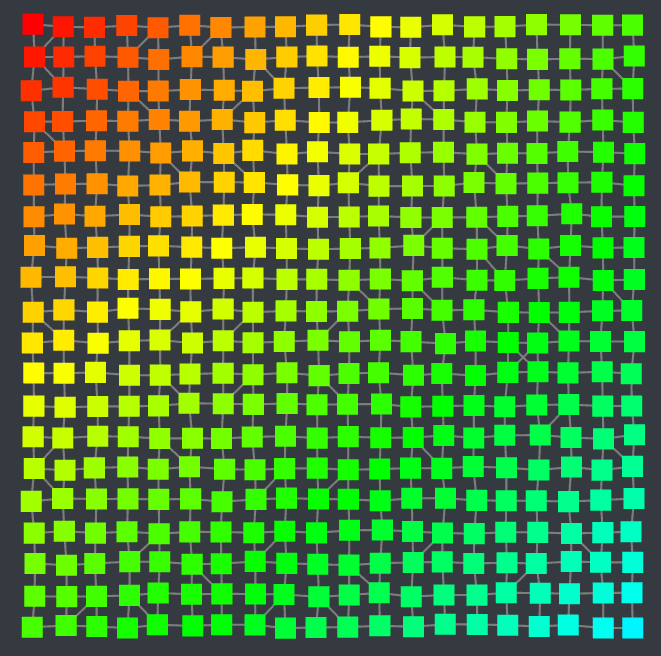
\includegraphics[width=0.2\textwidth]{img/gradient-scafi.png}
	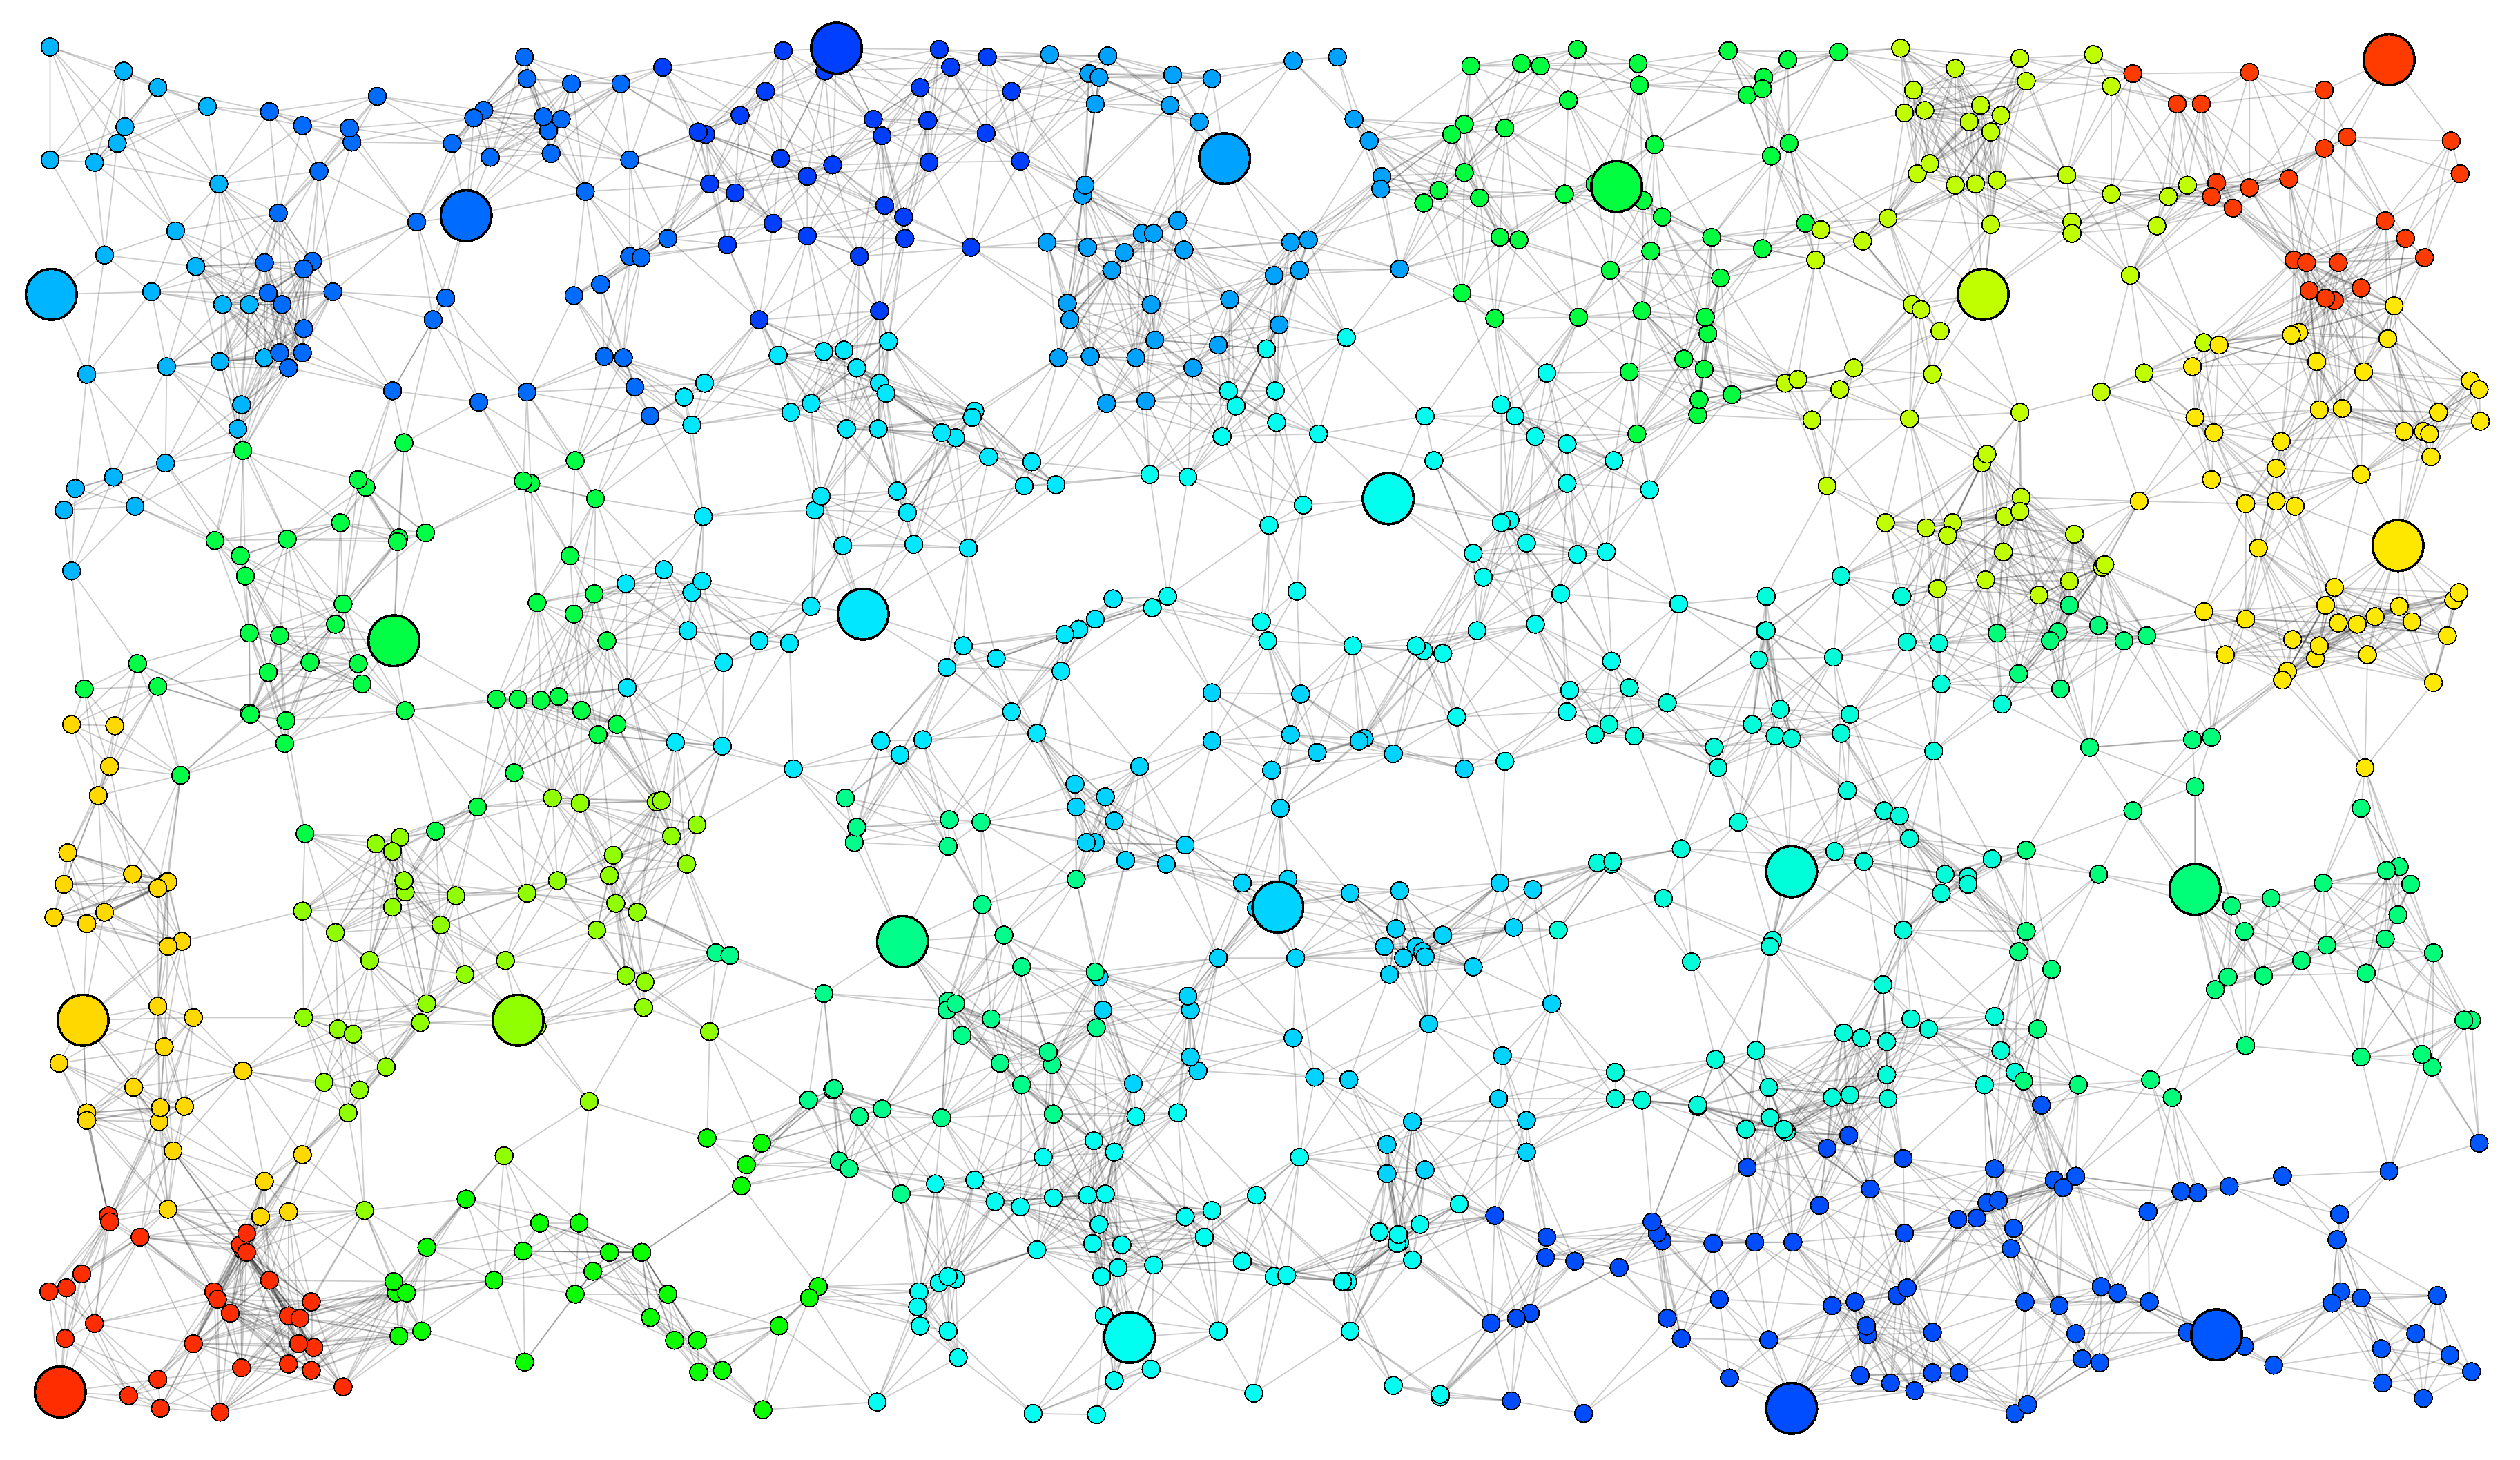
\includegraphics[width=0.35\textwidth]{img/scr-result.png}
	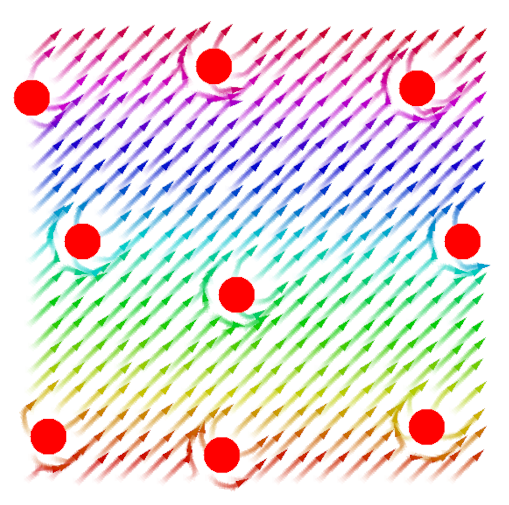
\includegraphics[width=0.215\textwidth]{img/obstacle-avoidance.png}
\end{center}
\end{frame}
\begin{frame}{ScaFi: Organization}
\centering
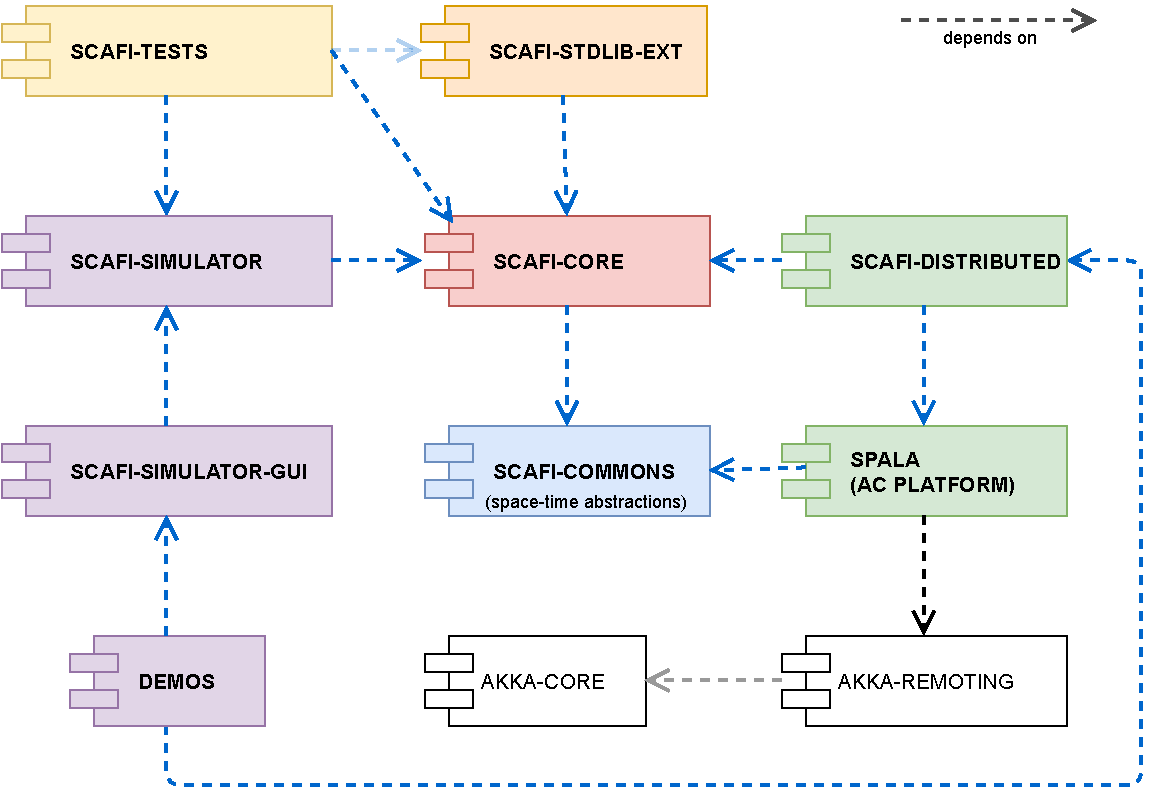
\includegraphics[width=0.9\textwidth]{img/scafi-project-org.pdf}
\end{frame}
\begin{frame}{ScaFi: Design}
\centering
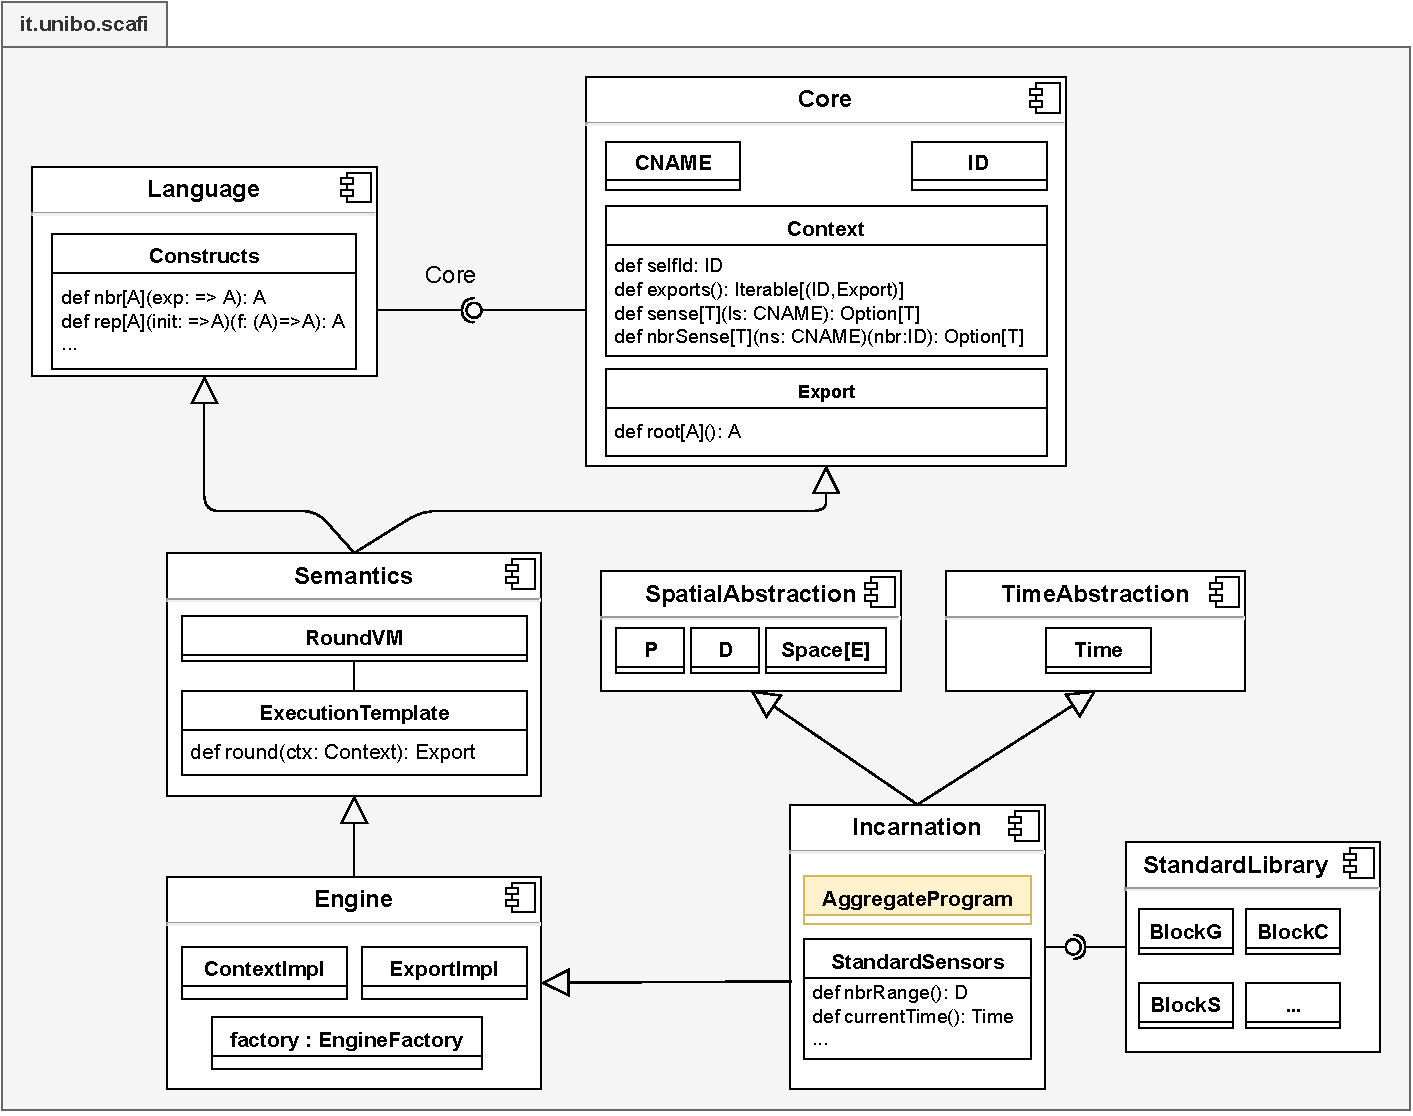
\includegraphics[width=0.8\textwidth]{img/scafi-design.drawio.pdf}
\end{frame}
\begin{frame}[fragile]{ScaFi: syntax as a core language/API}

	\begin{mycode}{}{}{}
trait Constructs {
	// the unique identifier of the local device 
	def mid(): ID
	
	// applies fun to the previous result, or to init at the first call
	def rep[A](init: A)(fun: (A) => A): A
	
	// evaluation of expr at the currently-considered neighbour
	def nbr[A](expr: => A): A
	
	// accumulates available evaluations of expr, with acc/init monoid
	def foldhood[A](init: => A)(acc: (A,A)=>A)(expr: => A): A
	
	// splits computation: th where cond is true, el everywhere/time else
	def branch[A](cond: => Boolean)(th: => A)(el: => A): A
	
	// perception of local sensor
	def sense[A](name: CNAME): A
	
	// perception of neighbourhood sensor
	def nbrvar[A](name: CNAME): A
	...
}
\end{mycode}
\end{frame}

\begin{frame}[fragile]{ScaFi: setup an aggregate application}
\begin{mycode}{}{}{}
package experiments
// STEP 1 Choose an incarnation (simulated or real)
import it.unibo.scafi.incarnations.BasicSimulationIncarnation._

// STEP 2 Define the aggregate program including the right libraries
class MyProgram extends AggregateProgram with Libs {
	// STEP 2.1 Define main logic of the program
	override def main(): Any = rep(0)(_ + 1)
}

// STEP 3 Platform/Node setup (both in simulation/real)

// STEP 3.1 in case of ScaFi simulation:
object SimulationRunner extends Launcher {
  Settings.Sim_ProgramClass = "experiments.MyAggregateProgram"
  Settings.ShowConfigPanel = true
  launch()
}
\end{mycode}
\end{frame}
\begin{frame}{An aggregate computing playground -- ScaFi Web!}
\centering
\url{https://scafi.github.io/web/}
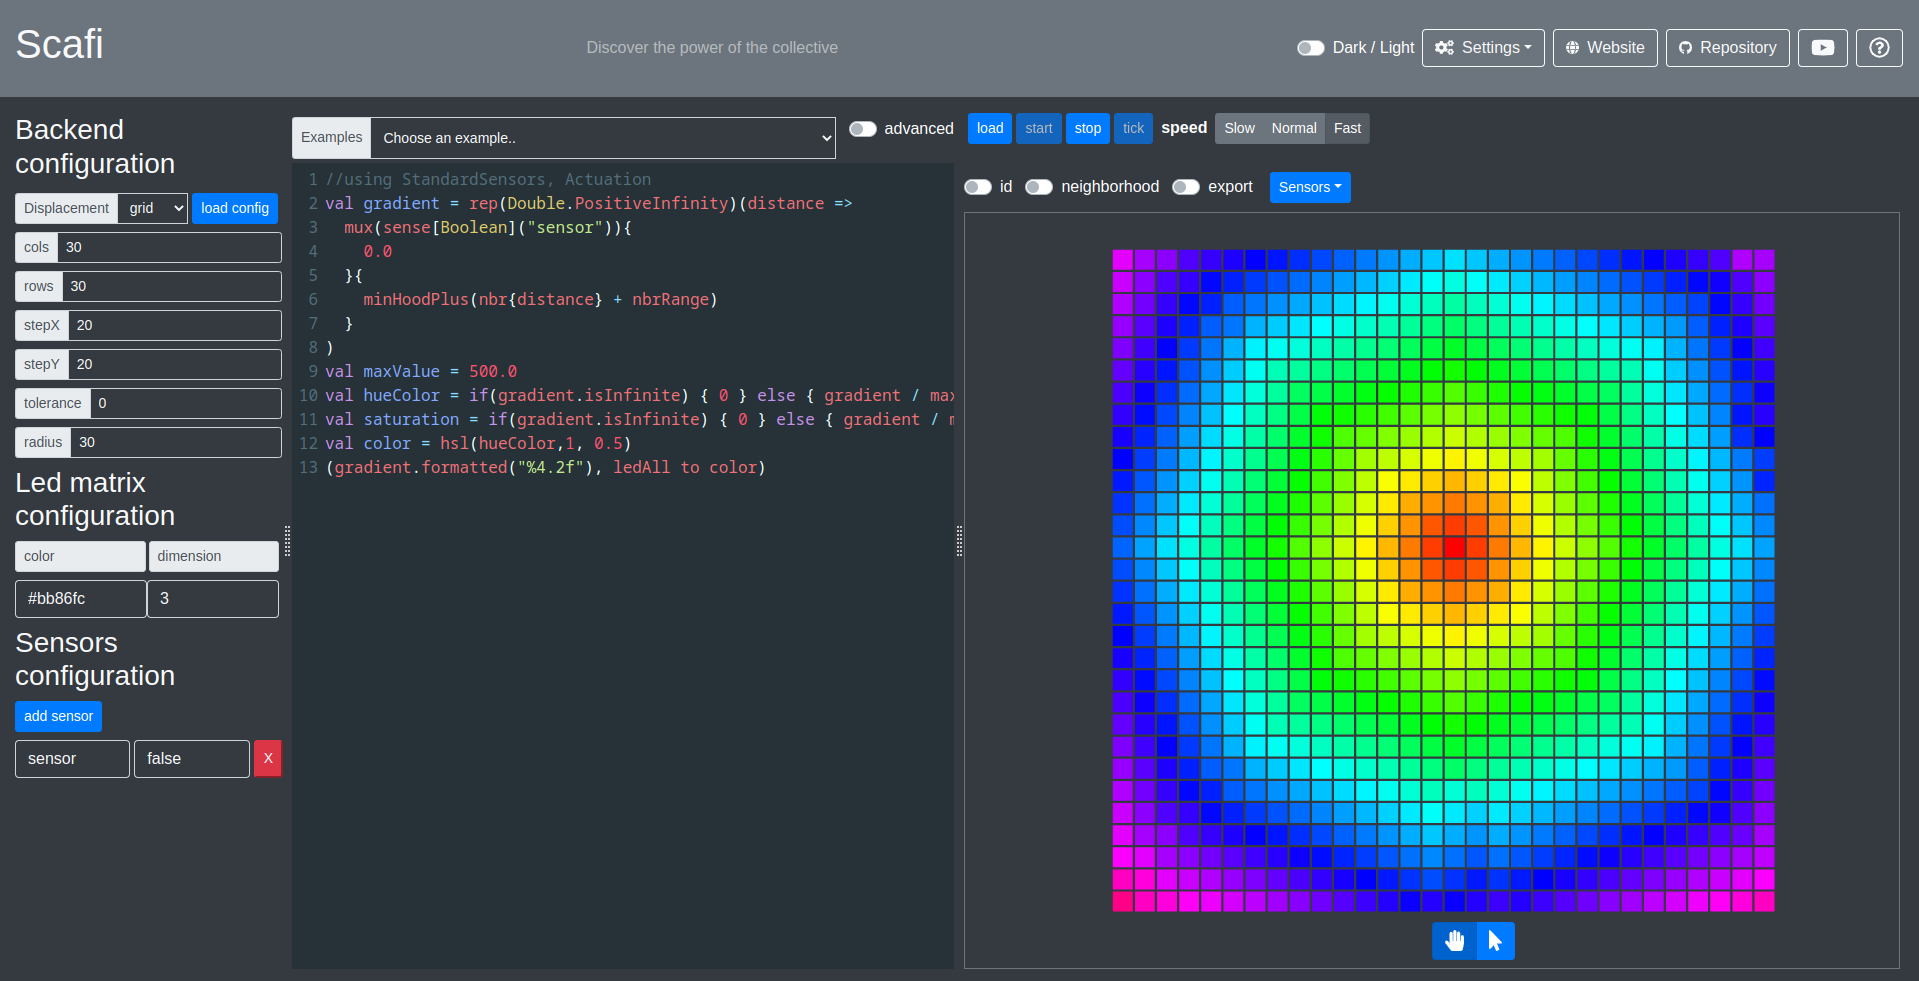
\includegraphics[width=\textwidth]{img/gradient-web.png}
\end{frame}

%\section{Aggregate Computing -- Research Profiles}
%\begin{frame}{Swarm Robotics}

%\end{frame}
%\begin{frame}{\st{Multi} Many agent reinforcement}
%\end{frame}

\begin{frame}[fragile]{Example 1: static constant field}

\begin{mycode}{}{}{}
// 1. Select the incarnation
import it.unibo.alchemist.model.scafi.ScafiIncarnationForAlchemist._

// 2. define your aggregate program by extending 'AggregateProgram'
class Example1 extends AggregateProgram {
  // 3. define the main method of the aggregate computing script
    override def main(): Int = 22
}
\end{mycode}

\imgv{0.6}{example1-static-const-field.png}

\end{frame}

\begin{frame}[fragile]{Example 3: sensor query}{\textbf{\texttt{mid()}} provides the device ID}

\begin{mycode}{}{}{}
// Code in the AggregateProgram's main method:
mid()
\end{mycode}

\imgv{0.7}{example3-mid.png}

\end{frame}


\begin{frame}[fragile]{Example 4: sensor query}{\textbf{\texttt{sense("name")}} reads the current value of a sensor}

\begin{mycode}{}{}{}
sense[Boolean]("source")
\end{mycode}

\imgv{0.7}{example4-source.png}

\end{frame}

\begin{frame}[fragile]{Example 5: neighbour interaction}{\textbf{\texttt{foldhood(i)(f)(e)}} aggregates with \texttt{f} the neighbours' values for \texttt{e}}

\begin{mycode}{}{}{}
// *Plus version does not consider the device itself in the neighbourhood
foldhoodPlus(0)((a,b) => a + b)(nbr(1))
\end{mycode}

\imgv{0.7}{example5-fold.png}

\end{frame}


\begin{frame}[fragile]{Example 6: stateful computations}{\textbf{\texttt{rep(i)(f)}} updates a value (initially \texttt{i}) through function \texttt{f}}

\begin{mycode}{}{}{}
rep(0){ _ + 1 }
\end{mycode}

\imgv{0.7}{example6-rep.png}

\end{frame}


\begin{frame}[fragile]{Example 8: self-healing gradient}{Field of minimum distances from source nodes}

\begin{mycode}{}{}{}
rep(Double.PositiveInfinity)(distance =>
    mux(sense[Boolean]("source")) {
      0.0
    } {
      minHoodPlus(nbr(distance) + nbrRange)
    }
  )
\end{mycode}

\imgv{0.7}{example8-gradient.png}

\end{frame}


\section{}

%===============================================================================

%/////////
\frame{\titlepage}
%/////////

%===============================================================================
\section*{\refname}
%===============================================================================

%%%%
\setbeamertemplate{page number in head/foot}{}
%/////////


\begin{frame}[allowframebreaks]{References}
\def\bibfont{\footnotesize}
\printbibliography
\end{frame}

%%%%%%%%%%%%%%%%%%%%%%%%%%%%%%%%%%%%%%%%%%%%%%%%%%%%%%%%%%%%%%%%%%%%%%%%%%%%%%%%
\end{document}
%%%%%%%%%%%%%%%%%%%%%%%%%%%%%%%%%%%%%%%%%%%%%%%%%%%%%%%%%%%%%%%%%%%%%%%%%%%%%%%%
